\documentclass[a4paper,11pt]{article}
\usepackage{hyperref}

\usepackage[T1]{fontenc}
\usepackage[utf8]{inputenc}
\usepackage{graphicx}
\usepackage{xcolor}
%\usepackage[margin=1in]{geometry}


\begin{document}

\title{FiveThirtyEight Riddler Express Solution}


\author{John Bullock}

\date{05/22/2020}

\graphicspath{{Images/}}

\maketitle
\section*{Problem Setup}

From the FiveThirtyEight problem setup:\newline

\textit{To share a cylindrical muffin equally with his two toddlers, Robert makes three vertical cuts in a “Y” pattern, producing three equal pieces.}

\textit{The next morning, his wife wants in on the fun. But before he can cut the muffin into quarters with an “X” pattern, one of his children suggests using an “A” pattern. If Robert were to produce equal fourths in this manner, what would be the ratio of length of the A’s middle bar to the radius of the muffin?}


\section*{Problem Solution}

To simplify the problem, we will examine the problem as making the "A" cut to divide a circle into four sections of equal area.  By observation of Figure \ref{fig:areas}, it appears that the "A" pattern cut divides a circle into two circular segments (Areas I and II), a triangle (Area III), and some irregular shape that vaguely resembles a trapezoid (Area IV).

\begin{figure}[htp]
    \centering
    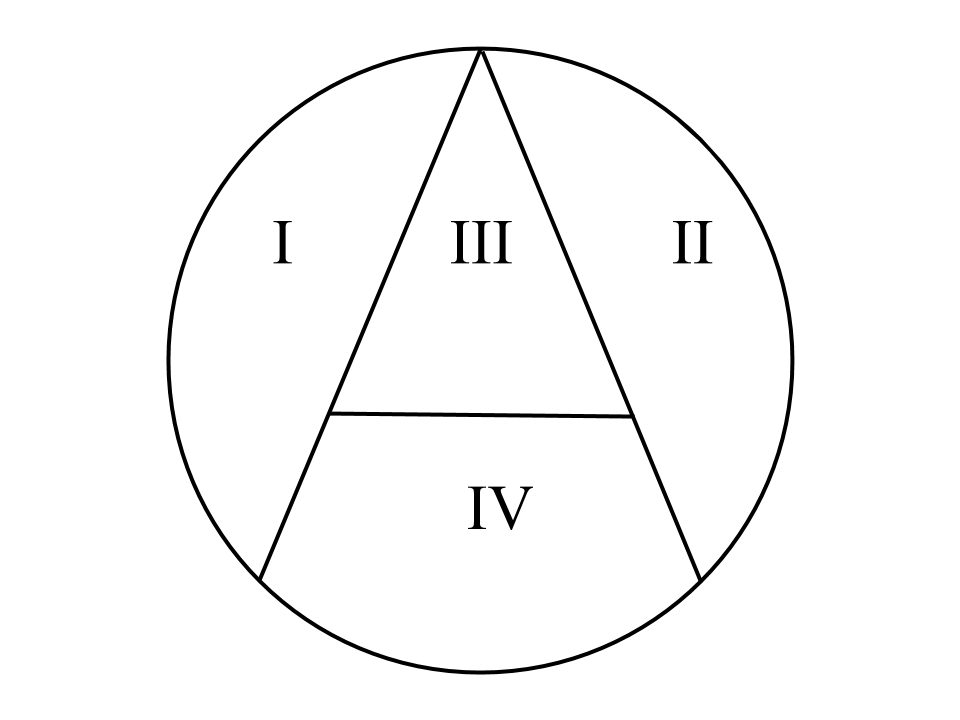
\includegraphics[width=6cm]{Images/2020_05_22_Riddler_Express.png}
    \caption{An "A" Pattern Cut of a Circle}
    \label{fig:areas}
\end{figure}

\subsection*{Circular Segment Area}

\hspace{\parindent}First, we can examine the case of the two circular segments made by the "A" pattern cut, represented by Areas I and II seen in Figure \ref{fig:segmentArea}.  To make a successful "A" cut that satisfies the problem requirement of $A_I=A_{II}=A_{III}=A_{IV}$, the only parameter that we can design is the angle $\theta$ seen in Figure \ref{fig:segmentArea} below.

\begin{figure}[htp]
    \centering
    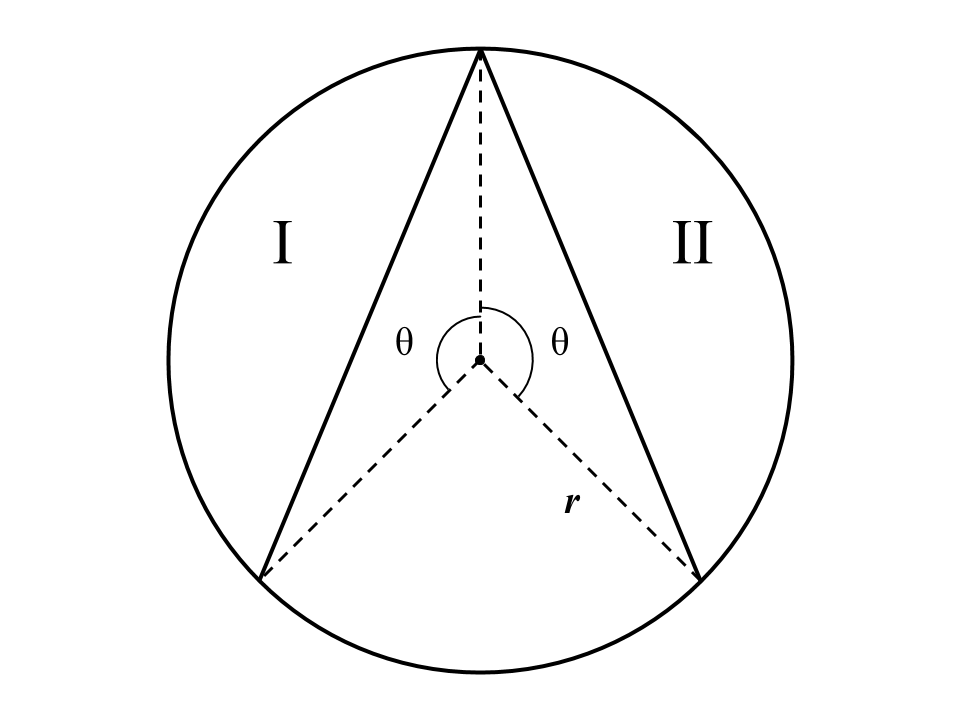
\includegraphics[width=6cm]{Images/2020_05_22_Riddler_Express_CircleSectors.png}
    \caption{The Circular Segments of the "A" Cut}
    \label{fig:segmentArea}
\end{figure}

It is known that the area of a circular segment that encompasses Areas I and II can be represented by the equation below, where $\theta$ is measured in radians.

\[A_I = A_{II} = \frac{r^2}{2}(\theta - \sin{\theta})\]


Since we are dividing the circle into four sections of equal area, Area I and Area II each must take up a quarter of the area of the whole circle.  This relationship can be used to solve for the value $\theta$ needed to satisfy $A_{I}=A_{II}=\frac{1}{4}A_{circle}$.


\[\frac{1}{4}\cdot A_{circle} = A_{I}\]
\[\frac{\pi}{4} \cdot r^2= \frac{r^2}{2}(\theta - \sin{\theta})\]
\[\frac{\pi}{2} = \theta - \sin{\theta}\]

This equation can't be solved analytically, but WolframAlpha found a numerical solution of $\theta \approx 2.30988$ radians.\newline\newline\newline

\subsection*{Triangular Area}

Next, we can start to find the area of the triangular area contained in Area III of Figure \ref{fig:areas}.  One approach to doing finding the triangular area in Area III is to find the inscribed angle $\alpha$ seen in Figure \ref{fig:alpha}, and using the following formula for computing the area of a triangle.
\[A_{III} = \frac{1}{2} \cdot l_{AB} \cdot l_{AC} \cdot \sin{\alpha}\]

\begin{figure}[htp]
    \centering
    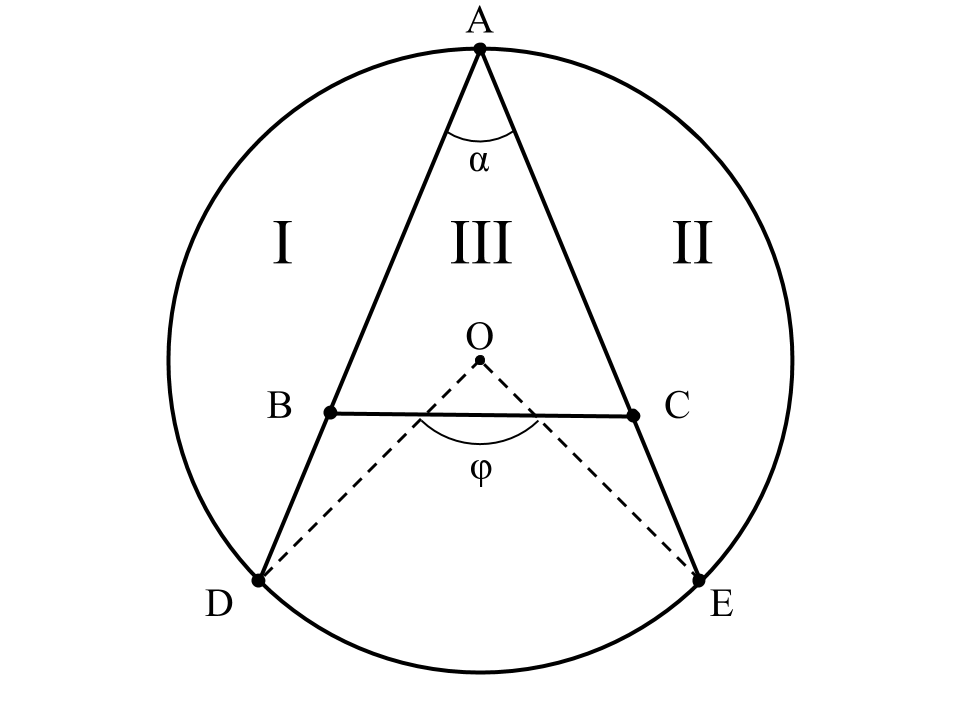
\includegraphics[width=6cm]{Images/Central_Angle.png}
    \caption{The Central and Inscribed Angles of the Circle}
    \label{fig:alpha}
\end{figure}

Notably, the inscribed angle $\alpha$ and the central angle $\phi$ share the same intercepted arc seen in Figure \ref{fig:alpha}, which means that they are related in the equation $\alpha = \frac{\phi}{2}$.

From Figure \ref{fig:phi}, we can see that the angle $\phi$ is related to $\theta$ from the equation $\phi = 2\pi - 2\theta$.  Substituting the two previously derived equations, we come up with an expression for inscribed angle $\alpha$ in terms of $\theta$.
\[\alpha = \pi - \theta\]
\[\alpha \approx 0.83171\]

\begin{figure}[htp]
    \centering
    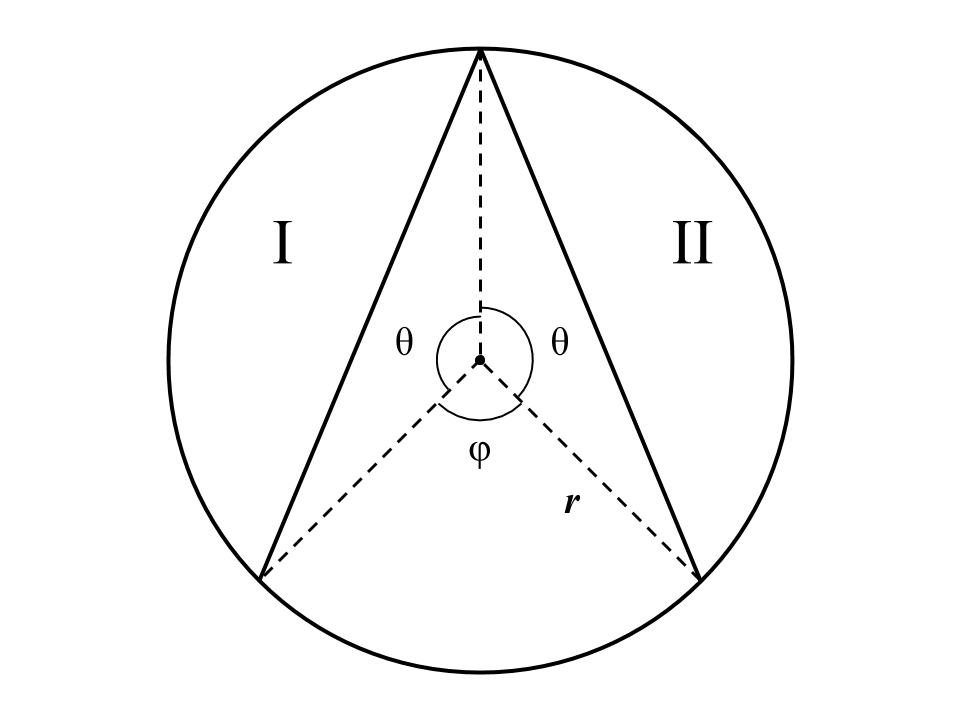
\includegraphics[width=6cm]{Images/2020_05_22_Riddler_Express_Phi.png}
    \caption{Defining Central Angle $\phi$ in Terms of $\theta$}
    \label{fig:phi}
\end{figure}

For simplicity, let's define $s=l_{AB}=l_{AC}$ and $b=l_{CB}$ as seen in Figure \ref{fig:triangle}.  We can define one more relationship between $s$ and $b$ from trigonometry, with $\frac{b}{2} = s \cdot \sin{\frac{\alpha}{2}}$. We now have all the necessary values for calculating the triangular area of Area III using the equation $A_{III} = \frac{1}{2} \cdot l_{AB} \cdot l_{AC} \cdot \sin{\alpha}$.  


\[A_{III} = \frac{1}{2} \cdot l_{AB} \cdot l_{AC} \cdot \sin{\alpha}\]
\[\frac{\pi}{4} \cdot r^2 = \frac{1}{2} \cdot l_{AB} \cdot l_{AC} \cdot \sin{\alpha}\]
\[\frac{\pi}{2} \cdot r^2 = s^2 \cdot \sin{\alpha}\]
\[r^2 = s^2 \cdot \frac{2}{\pi} \cdot \sin{\alpha}\]
\[r =s \cdot \sqrt{\frac{2}{\pi} \cdot \sin{\alpha}}\]

Now we use the derived equation $\frac{b}{2} = s \cdot \sin{\frac{\alpha}{2}}$ to come up with the substitution $s =\frac{b}{2\sin{\frac{\alpha}{2}}}$.

\[r =\frac{b}{2\sin{\frac{\alpha}{2}}} \cdot \sqrt{\frac{2}{\pi} \cdot \sin{\alpha}}\]
\[\frac{b}{r} = 2\sin{\frac{\alpha}{2}} \cdot \sqrt{\frac{\pi}{2\sin{\alpha}}}\]

Using the calculated value of $\alpha \approx 0.83171 $ radians, we can approximate the ratio of $\frac{b}{r}$ as:
\[\frac{b}{r} \approx 1.1779\]


\begin{figure}[htp]
    \centering
    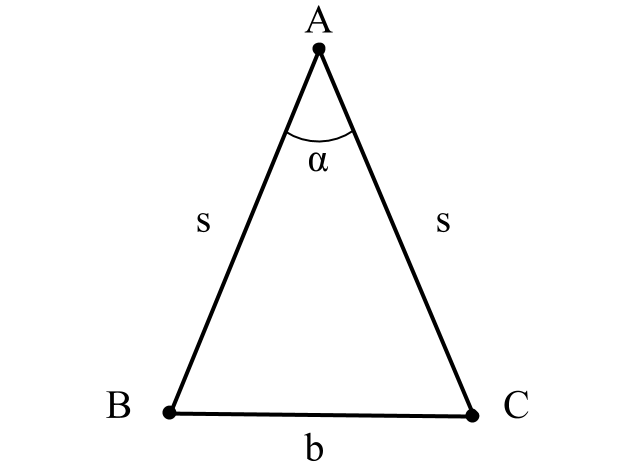
\includegraphics[width=6cm]{Images/Triangle_3_Area.png}
    \caption{Dimensions for the Area III Triangle}
    \label{fig:triangle}
\end{figure}



\end{document}
